  \let\negmedspace\undefined
\let\negthickspace\undefined
\documentclass[journal]{IEEEtran}
\usepackage[a5paper, margin=10mm, onecolumn]{geometry}
\usepackage{lmodern} % Ensure lmodern is loaded for pdflatex
\usepackage{tfrupee} % Include tfrupee package

\setlength{\headheight}{1cm} % Set the height of the header box
\setlength{\headsep}{0mm}     % Set the distance between the header box and the top of the text

\usepackage{gvv-book}
\usepackage{gvv}
\usepackage{cite}
\usepackage{amsmath,amssymb,amsfonts,amsthm}
\usepackage{algorithmic}
\usepackage{graphicx}
\usepackage{textcomp}
\usepackage{xcolor}
\usepackage{txfonts}
\usepackage{listings}
\usepackage{enumitem}
\usepackage{mathtools}
\usepackage{gensymb}
\usepackage{comment}
\usepackage[breaklinks=true]{hyperref}
\usepackage{tkz-euclide} 
\usepackage{listings}                                      
\def\inputGnumericTable{}                                 
\usepackage[latin1]{inputenc}                                
\usepackage{color}                                            
\usepackage{array}                                            
\usepackage{longtable}
\usepackage{multicol}
\usepackage{calc}                                             
\usepackage{multirow}                                         
\usepackage{hhline}                                           
\usepackage{ifthen}                                           
\usepackage{lscape}
\begin{document}

\bibliographystyle{IEEEtran}
\vspace{3cm}

\title{12.9.7.15}
\author{EE24BTECH11024 - G. Abhimanyu Koushik}
% \maketitle
% \newpage
% \bigskip
{\let\newpage\relax\maketitle}

\renewcommand{\thefigure}{\theenumi}
\renewcommand{\thetable}{\theenumi}
\setlength{\intextsep}{10pt} % Space between text and floats


\numberwithin{equation}{enumi}
\numberwithin{figure}{enumi}
\renewcommand{\thetable}{\theenumi}


\textbf{Question}:\newline
The population of a village increases continuously at the rate proportional to the
number of its inhabitants present at any time. If the population of the village was
20,000 in 1999 and 25,000 in the year 2004, what will be the population of the
village in 2009?
\newline
\textbf{Solution: }
\begin{table}[h!]    
  \centering
  \begin{tabular}[12pt]{ |c| c|}
    \hline
    \textbf{Variable} & \textbf{Description}\\
    \hline
    $n$ & Order of given differential equation\\
    \hline
    $a_i$ & Coeefficient of $i$th derivative of the function in the equation\\
    \hline
    $c$ & constant in the equation\\
    \hline
    $y^i$ & $i$th derivative of given function\\
    \hline
    $\vec{y}\brak{t}$ & $\myvec{c \\ y\brak{t} \\ y^\prime\brak{t} \\ \vdots \\ y^{n-1}\brak{t}}$\\
    \hline
    $h$ & stepsize, taken to be 0.001\\
    \hline
    $u\brak{x}$ & Unit step function\\
    \hline
    \end{tabular}

  \caption{Variables Used}
  \label{tab1.1.2.2}
\end{table}
\newline
Theoritical Solution:\\
Laplace Transform definition\\
\begin{align}
	\mathcal{L}\brak{f\brak{t}} = \int_{0}^{\infty}e^{-st}f\brak{t}dt
\end{align}
Properties of Laplace tranform
\begin{align}
	\mathcal{L}\brak{y^{\prime}} &= s\mathcal{L}\brak{y} -y\brak{0}\\
	\mathcal{L}\brak{1} &= \frac{1}{s}\\
	\mathcal{L}\brak{cf\brak{t}} &= c\mathcal{L}\brak{f\brak{t}}\\
	\mathcal{L}\brak{f\brak{t}} = F\brak{s} &\implies \mathcal{L}\brak{e^{at}f\brak{t}} = F\brak{s-a}	
\end{align}
Applying the properties to the given equation
\begin{align}
	y^{\prime} &= k_{0}y\\
	\mathcal{L}\brak{y^\prime} - \mathcal{L}\brak{k_{0}y}&= 0\\
	s\mathcal{L}\brak{y} - y\brak{0} - k_{0}\mathcal{L}\brak{y} &= 0\\
	\mathcal{L}\brak{y} &= \frac{y\brak{0}}{s - k_{0}}\\
	y &= y\brak{0}e^{k_{0}x}u\brak{x}
\end{align}
Taking 1999 to be the initial year, we get $y\brak{0} = 20000$ and $y\brak{5} = 25000$\\
Substituting the initial conditions gives
\begin{align}
	y\brak{0} &= 20000\\
	y\brak{5} &= 25000\\
	20000e^{5k_{0}} &= 25000\\
	e^{5k_{0}} &= \frac{5}{4}\\
	5k_{0} &= \ln{\frac{5}{4}}\\
	k_{0} &= \frac{1}{5}\ln{\frac{5}{4}}
\end{align}
The theoritical solution is 
\begin{align}
	f\brak{x} &= 20000e^{\frac{1}{5}\brak{\ln{\frac{5}{4}}}x}u\brak{x}\\
	f\brak{x} &= 20000\brak{\frac{5}{4}}^{\frac{x}{5}}u\brak{x	}
\end{align}
Substituting $x=10$ gives 31250
\newline
Computational Solution:\newline
First we have to find the $k$ value in the differential equation, for that
\begin{align}
	y\brak{t+h} &= y\brak{t} + hy^\prime\brak{t}\\
	y\brak{t+h} &= y\brak{t} + hk_{0}y\brak{t}\\
	y\brak{t+2h} &= y\brak{t+h} + hk_{0}y\brak{t+h}\\
	y\brak{t+2h} &= y\brak{t} + hk_{0}y\brak{t} + hk_{0}\brak{y\brak{t} + hk_{0}y\brak{t}}\\
	y\brak{t+2h} &= \brak{1+hk_{0}}^2y\brak{t}
\end{align}
Similarly
\begin{align}
	y\brak{t+nh} &= \brak{1+hk_{0}}^ny\brak{t}
\end{align}
Subtituting the initial condition and value of $h$ gives
\begin{align}
	y\brak{5} &= \brak{1+0.001k_{0}}^{5000}y\brak{0}\\
	25000 &= 20000\brak{1+0.001k_{0}}^{5000}\\
	\brak{\frac{5}{4}}^{\frac{1}{5000}} - 1 &= 0.001k_{0}\\
	k_{0} &= \frac{\brak{\frac{5}{4}}^{\frac{1}{5000}} - 1}{0.001}\\
	k_{0} &\approx 0.04462
\end{align}
Consider the given linear differential equation
\begin{align}
	a_{n}y^n + a_{n-1}y^{n-1} + \dots + a_{1}y^\prime + a_{0}y + c = 0
\end{align}
Then
\begin{align}
	y^{\prime}\brak{t} = \lim_{h\to 0}\frac{y\brak{t+h} - y\brak{t}}{h}\\
	y\brak{t+h} = y\brak{t} + hy^{\prime}\brak{t}
\end{align}
Similarly
\begin{align}
	y^{i}\brak{t+h} &= y^{i}\brak{t} + hy^{i+1}\brak{t}\\
	y^{n-1}\brak{t+h} &= y^{n-1}\brak{t} + hy^{n}\brak{t}\\
	y^{n-1}\brak{t+h} &= y^{n-1}\brak{t} + h\brak{-\frac{a_{n-1}}{a_n}y^{n-1}-\frac{a_{n-2}}{a_n}y^{n-2} - \dots -\frac{a_{0}}{a_n}y - \frac{c}{a_n}}
\end{align}
Where i ranges from 0 to $n-1$\\
\begin{align}
	\vec{y}\brak{t+h} &= \vec{y}\brak{t} + \myvec{0 & 0 & 0 & 0 & \dots & 0 & 0\\ 0 & 0 & 1 & 0 & \dots & 0 & 0\\0 & 0 & 0 & 1 & \dots & 0 & 0\\\vdots & \vdots & \vdots & \vdots& \ddots & \vdots & \vdots\\
	0 & 0 & 0 & 0 & \dots & 0 & 1\\-\frac{1}{a_n} & -\frac{a_0}{a_n} & -\frac{a_1}{a_n} & -\frac{a_2}{a_n} & \dots & -\frac{a_{n-2}}{a_n} & -\frac{a_{n-1}}{a_n}}\brak{h\vec{y}\brak{t}}\\
	\vec{y}\brak{t+h} &= \myvec{1 & 0 & 0 & 0 & \dots & 0 & 0\\ 0 & 1 & h & 0 & \dots & 0 & 0\\0 & 0 & 1 & h & \dots & 0 & 0\\\vdots & \vdots & \vdots & \vdots& \ddots & \vdots & \vdots\\
	0 & 0 & 0 & 0 & \dots & 1 & h\\-\frac{h}{a_n} & -\frac{a_0h}{a_n} & -\frac{a_1h}{a_n} & -\frac{a_2h}{a_n} & \dots & -\frac{a_{n-2}h}{a_n} & 1-\frac{a_{n-1}h}{a_n}}\brak{\vec{y}\brak{t}}
\end{align}
Discretizing the steps gives us
\begin{align}
	\vec{y}_{k+1} = \myvec{1 & 0 & 0 & 0 & \dots & 0 & 0\\ 0 & 1 & h & 0 & \dots & 0 & 0\\0 & 0 & 1 & h & \dots & 0 & 0\\\vdots & \vdots & \vdots & \vdots& \ddots & \vdots & \vdots\\
	0 & 0 & 0 & 0 & \dots & 1 & h\\-\frac{h}{a_n} & -\frac{a_0h}{a_n} & -\frac{a_1h}{a_n} & -\frac{a_2h}{a_n} & \dots & -\frac{a_{n-2}h}{a_n} & 1-\frac{a_{n-1}h}{a_n}}\brak{\vec{y}_{k}}
\end{align}
where $k$ ranges from 0 to number of data points with $y^{i}_0$ being the given initial condition and vector $\vec{y}_0 = \myvec{c\\y\brak{0}\\y^\prime\brak{0}\\\vdots\\y^{n-1}\brak{0}}$\\
for finding the value of $a_0$, we wil substitute the initial conditions as in theoritical solution\\
For the given question\\
\begin{align}
	\vec{y}_{k+1} = \myvec{1 & 0\\ -h & 1+hk_0}\vec{y}_k
\end{align}
Record the $y_k$ for 
\begin{align}
x_k =lowerbound+kh
\end{align}
and then plot the graph. The result will be as given below.
\begin{figure}[h!]
   \centering
   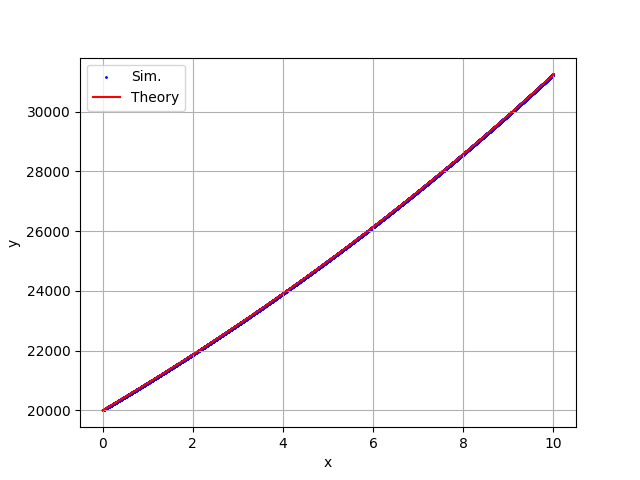
\includegraphics[width=\columnwidth]{figs/fig.png}
   \caption{Comparison between the Theoritical solution and Computational solution}
   \label{stemplot}
\end{figure}
\end{document}  
